
\documentclass[
	12pt,				
	oneside,
	a4paper,
	english,
	brazil,
	]{abntex2}

\usepackage{estilos/pacotes}

%Define Fonte
\setmainfont[Path=./fonts/,
    BoldItalicFont=calibriz.ttf,
    BoldFont      =calibrib.ttf,
    ItalicFont    =calibrii.ttf]{calibri.ttf}  % Fonte Calibri
\renewcommand{\ABNTEXchapterfont}{\normalfont}

\usepackage{estilos/dissertacao_tese} 								% Customizacoes

\usepackage{estilos/informacao}

% informações do PDF
\makeatletter
\hypersetup{
     	%pagebackref=true,
		pdftitle={\@title}, 
		pdfauthor={\@author},
    	pdfsubject={\imprimirpreambulo},
	    pdfcreator={LaTeX with abnTeX2},
		pdfkeywords={abnt}{latex}{abntex}{abntex2}, 
		bookmarksdepth=4
}
\makeatother
% --- 

% O tamanho do parágrafo é dado por:
\setlength{\parindent}{1.25cm}

% Controle do espaçamento entre um parágrafo e outro:
\setlength{\parskip}{0.2cm}  % tente também \onelineskip

% Compila o índice
\makeindex


% Início do documento
\begin{document}


\selectlanguage{brazil}

% Retira espaço extra obsoleto entre as frases.
\frenchspacing 


% ----------------------------------------------------------
% ELEMENTOS PRÉ-TEXTUAIS
% ----------------------------------------------------------

\pretextual

\imprimircapa{}
\pagenumbering{roman}
%\textual
\imprimirfolhaderosto{}
\begin{fichacatalografica}
    \begin{flushleft}
    \large\textbf{Ficha Catalográfica}
    \end{flushleft}
	%\vspace*{\fill}					% Posição vertical
	\begin{flushleft}
	Ficha catalográfica elaborada pela Biblioteca do Centro Universitário SENAI Cimatec
	\end{flushleft}
	\begin{center}					% Minipage Centralizado
	\hrule
	\begin{minipage}[c][5cm]{13.5cm}		% Largura
	\small
	\imprimirautorsobrenome
	%Sobrenome, Nome do autor
	
	\hspace{0.5cm} 
	\imprimirtitulo\hspace{1mm}/ \imprimirautor. -- \imprimirlocal, \imprimirdata. \thelastpage p. 
	
	\hspace{0.5cm} 
	1. Palavra-chave1. 2. Palavra-chave2. 3. Palavra-chave3. I. Título. \\
	
	\hspace{0.5cm} 
	CDD XXX.XXXX
	
	\end{minipage}
	\hrule
	\end{center}
\end{fichacatalografica}
\begin{folhadeaprovacao}

  \begin{center}
    {\ABNTEXchapterfont\Large\imprimirautor}

    \begin{center}
      \ABNTEXchapterfont\Large\imprimirtitulo
    \end{center}
   \end{center}
   
        
   \begin{flushright}
    Aprovada em xx de xxxx de 20XX. \\
   \end{flushright}
   
   
   \begin{flushleft}
   \textbf{Banca Examinadora: }
   \end{flushleft}
   \hfill \break
   \hrule
   \begin{flushleft}
    \textbf{\imprimirorientador\hspace{1mm}-- Orientador} \\
    %Doutor em xxxxxx pela Universidade de xxxxxx, cidade, País \\
    Doutor em XXX pela Universidade xxxxxx, Cidade, País \\
    Vinculado ao Centro Universitário SENAI CIMATEC
   \end{flushleft}
   
   \hfill \break
   \hrule
   \begin{flushleft}
    \textbf{\imprimircoorientador\hspace{1mm}-- Coorientador} \\
    Doutor em XXX pela Universidade xxxxxx, Cidade, País \\
    Vinculado a/ao Instituição do Coorientador
   \end{flushleft}
   
   \hfill \break
   \hrule
   \begin{flushleft}
    \textbf{Membro externo da Banca} \\
    Doutor em XXX pela Universidade de xxxxxx, Cidade, País \\
    Instituição do membro da banca
   \end{flushleft}
   
   \hfill \break
   \hrule 
   
    \begin{flushleft}
    \textbf{Membro externo da Banca}  \\
    Doutor em XXX pela Universidade de xxxxxx, Cidade, País \\
    Instituição do membro da banca
   \end{flushleft}
   
\end{folhadeaprovacao}
\begin{dedicatoria}
   \vspace*{\fill}
    \hspace{9cm} Dedico este trabalho a ...
    \vspace*{3cm}
\end{dedicatoria}
\begin{agradecimentos}
    
\end{agradecimentos}
\setlength{\absparsep}{18pt}
\begin{resumo}
  \noindent
  
  \textit{\textcolor{red}{O Resumo apresenta de forma concisa os pontos relevantes do trabalho. Deve ser estruturado da seguinte forma:  deve conter uma pequena introdução do trabalho que demostre a justificativa, objetivo do estudo, metodologia empregada de forma geral, principais resultados alcançados e conclusão. Deve ver apresentado em parágrafo único e conter de 150 a 500 palavras, conforme a ABNT NBR 6028.}}
  
  \hfill \break
  \textbf{Palavras-chaves:} Palavra-chave 1; Palavra-Chave 2; Palavra-Chave 3; \textit{\textcolor{red}{(inserir de 3 a 6 palavras-chave (Separadas por ponto)}}
\end{resumo}


\setlength{\absparsep}{18pt}
\renewcommand*\resumoatitlename{Abstract}
\begin{resumo}[Abstract]
  \begin{otherlanguage*}{english}
    \lipsum[1-1]

   \vspace{\onelineskip}
 
   \noindent 
   \textbf{Keywords:} Keyword 1; Keyword 2; Keyword 3; \textit{\textcolor{red}{(inserir de 3 a 6 palavras-chave (Separadas por ponto)}}
 \end{otherlanguage*}
\end{resumo}


\addcontentsline{toc}{chapter}{\listtablename}
\pdfbookmark[0]{\listtablename}{lot}
\listoftables*
\cleardoublepage
\renewcommand{\listfigurename}{Lista de Figuras}
	\pdfbookmark[0]{\listfigurename}{lof}
	\normalsize
	\listoffigures*
	\cleardoublepage
% ABNT NBR 10719:2015
% Lista de abreviaturas e siglas
% Elemento opcional. Consiste na relação alfabética das abreviaturas e siglas utilizadas no relatório, seguidas das palavras ou expressões correspondentes grafadas por extenso. Recomenda-se a elaboração de lista própria para cada tipo.
% EXEMPLO
% ABNT Associação Brasileira de Normas Técnicas
%------------------------------------------------
\cleardoublepage
\markboth{\nomname}{\nomname}

\makeatletter 
\renewcommand{\nomname}{Lista de Siglas}\@starttoc{las}
%\renewcommand*{\pagedeclaration}[1]{\dotfill \hyperpage{#1}}
\renewcommand*{\pagedeclaration}[1]{}
\newcommand{\abreviatura}[2]{\addcontentsline{las}{sig}{\numberline{#1}{#2}}}

\makeatother  

\begin{siglas}
\item[Adam] \textit{Adaptive Moment Estimation}
\item[AE] \textit{Autoencoder}
\item[AG] Algoritmo Genético
\item[CIG] \textit{Common-image Gather}
\item[CNN] \textit{Convolutional Neural Network}
\item[CRF] \textit{Conditional Random Field}
\item[ELU] \textit{Exponential Linear Unit}
\item[FCN] \textit{Fully Convolutional Network}
\item[FWI] \textit{Full Waveform Inversion}
\item[GPU] \textit{Graphical Processing Unit}
\item[Leaky ReLU] \textit{Leaky Rectified Linear Unit}
\item[MAE] \textit{Mean Absolute Error}
\item[MSE] \textit{Mean Squared Error}
\item[PCA] \textit{Principal Component Analysis}
\item[PReLU] \textit{Parametric Rectified Linear Unit}
\item[PSO] \textit{Particle Swarm Optimization}
\item[RAM] \textit{Random Access Memory}
\item[ReLU] \textit{Rectified Linear Unit}
\item[RTM] \textit{Reverse-Time Migration}
\item[SGD] \textit{Stochastic Gradient Descent}
\item[VAE] \textit{Variational Autoencoder}

\end{siglas}

\cleardoublepage
\makeatletter
\@mkboth{\MakeUppercase\nomname}{\MakeUppercase\nomname}%
\makeatother
  
\printnomenclature[3cm]

\pdfbookmark[0]{\contentsname}{toc}

\tableofcontents*  	
\cleardoublepage

\setlength\beforechapskip{-24pt}
\setlength\afterchapskip{12pt}


% ------------------
% ELEMENTOS TEXTUAIS
% ------------------
\textual
\pagenumbering{arabic}

\chapter{Introdução}
\label{ch:introducao}

\textit{\textcolor{red}{Sugere-se apresentar um texto adequadamente conciso, com a contextualização e justificativa do tema do trabalho. Importante que o candidato traga de forma geral, e contextualizada, a importância do tema da pesquisa, citar trabalhos relevantes já desenvolvidos. Adicionalmente, apresentar no último parágrafo da Introdução, antes do item objetivo, de forma conectada, a justificativa do estudo, ressaltando os impactos do mesmo.}}

\textit{\textcolor{red}{O texto deve evitar o aprofundamento ou detalhamento. A introdução deve contextualizar, apresentar os problemas, deficiências ou oportunidades de melhoria e justificar os objetivos a serem apresentados na sequencia.}}

Os textos em \textit{\textcolor{red}{vermelho e itálico}} são mais sobre a parte de orientação para preenchimento de cada tópico.

\begin{figure}[!h]
    \caption{Exemplo de imagem.}
    \centering
    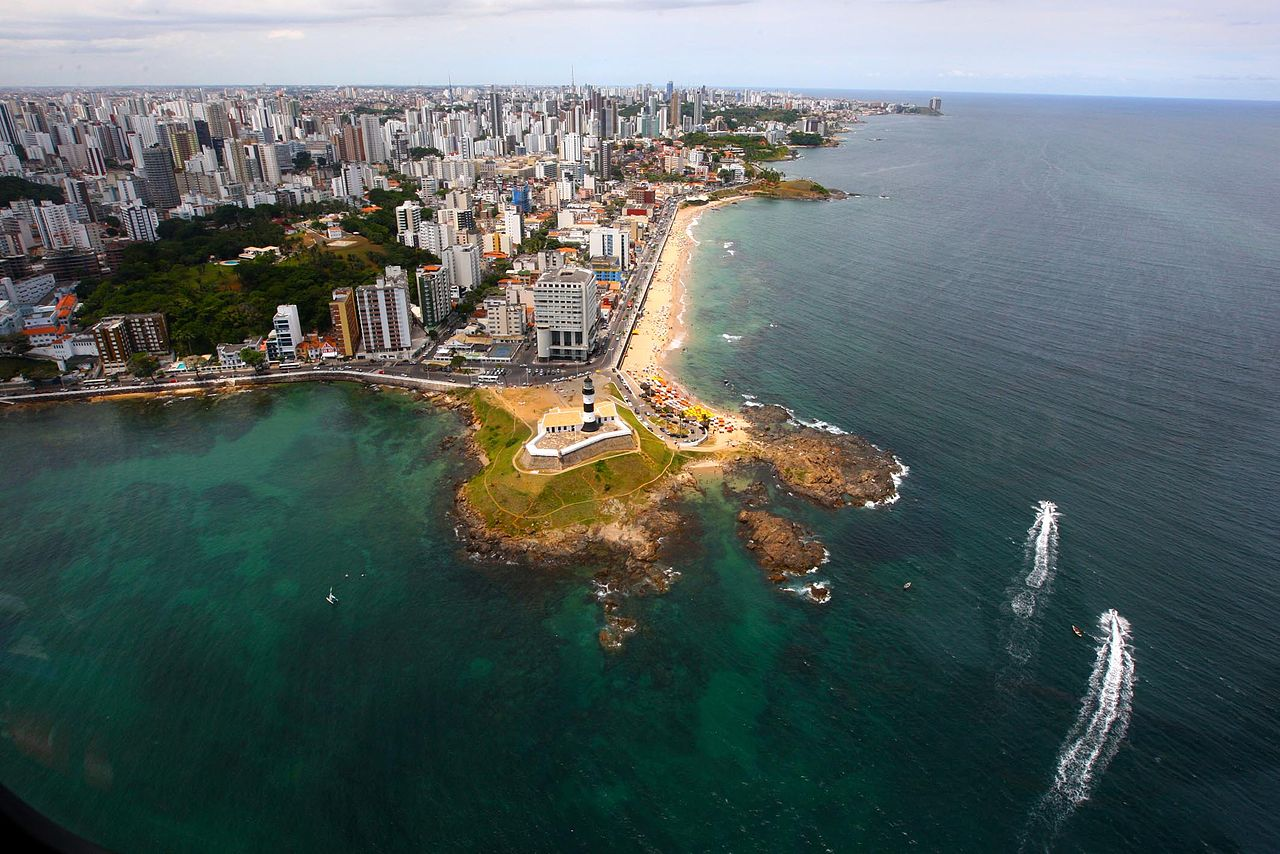
\includegraphics[width=0.6\textwidth]{images/farol_da_barra.jpg}
    \legend{Fonte: \cite{h2tp46-17}}
    \label{fig:seismic_acq}
\end{figure}

\lipsum[1-1]

\begin{figure}[!h]
    \caption{Exemplo com sub-imagem.}
    \centering
    \subfigure[Sub-imagem 1]{
      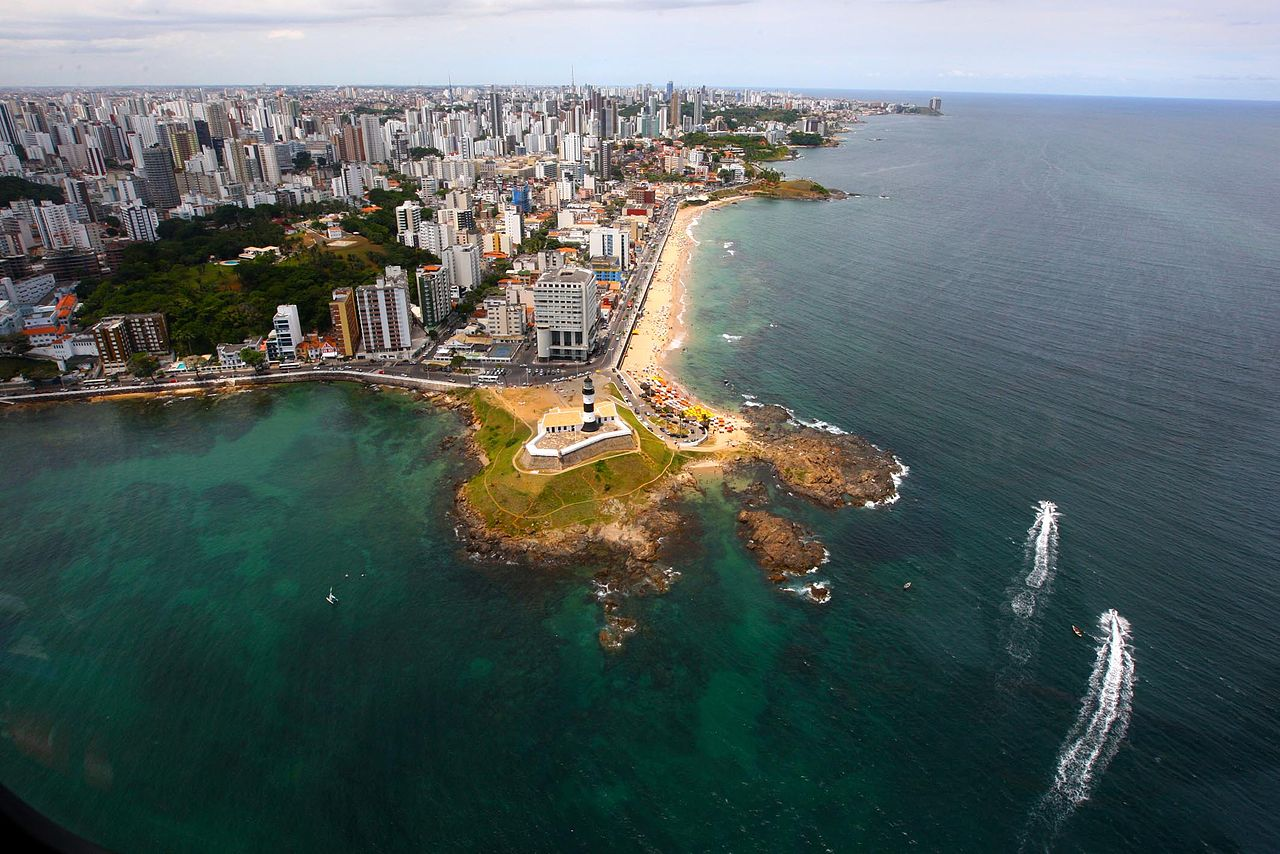
\includegraphics[width=.45\textwidth]{images/farol_da_barra.jpg}
      \label{fig:fig_exemplo_subimagem_1}
     }%
     \subfigure[Sub-imagem 2]{
      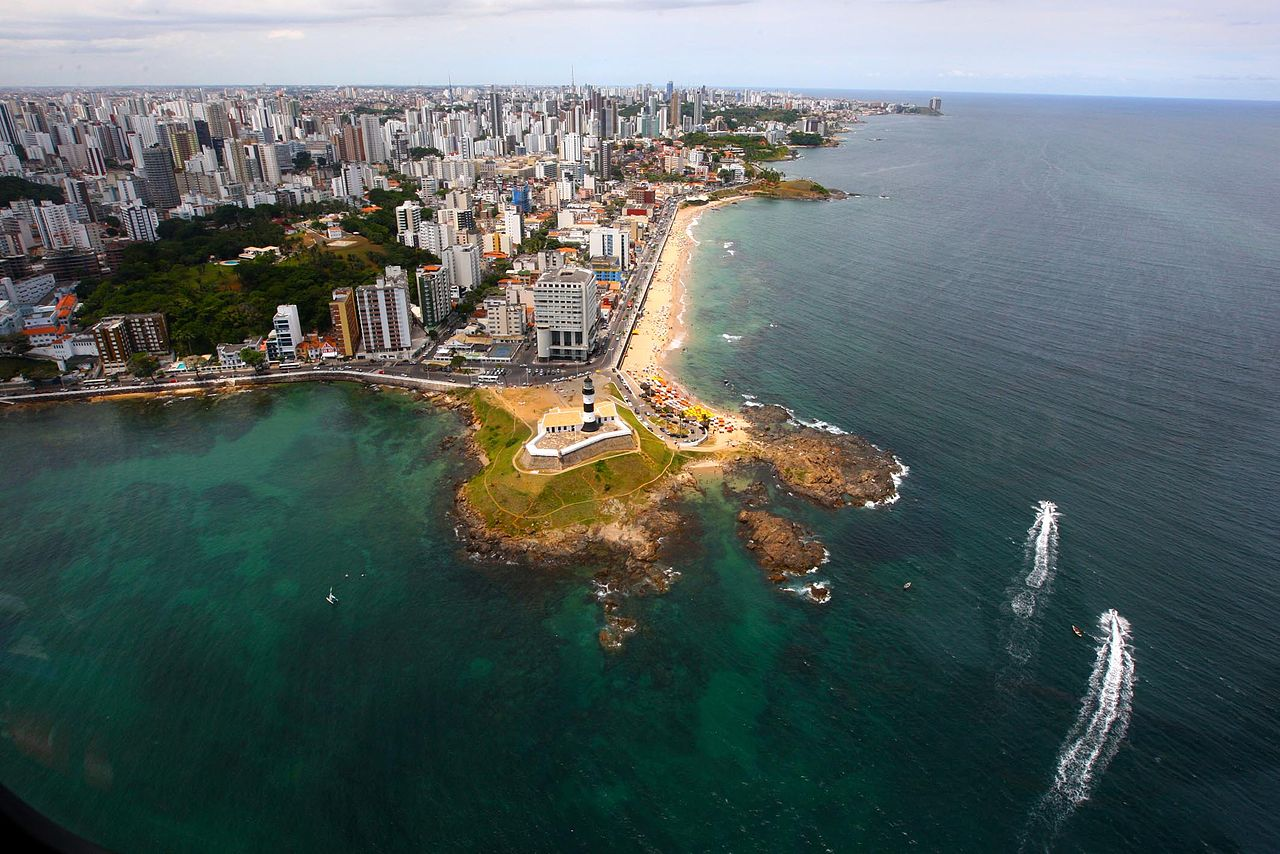
\includegraphics[width=.45\textwidth]{images/farol_da_barra.jpg}
      \label{fig:fig_exemplo_subimagem_2}
     }%
    \legend{Fonte: autoria própria.}
    \label{fig:fig_exemplo_subimagem}
\end{figure}

\lipsum[2-2]

\begin{enumerate}
    \item Item 1... ;
    \item Item 2... .
\end{enumerate}

\lipsum[3-3]

\section{Objetivo}
\label{section:objetivo}

\textit{\textcolor{red}{Apresentar o objetivo geral da Tese ou dissertação. Este precisa estar bem conectado com título do trabalho.}} O objetivo deste trabalho é...

\section{Objetivos Específicos}
\textit{\textcolor{red}{Apresentar os objetivos específicos da tese ou dissertação (em tópicos) – Lembre-se que TODOS os objetivos específicos devem ser respondidos na conclusão. Use uma sequência adequada que represente a apresentação de seus resultados.}}
Para alcançar o objetivo do trabalho, foi proposto como objetivos específicos:
\begin{enumerate}
    \item Realizar...;
    \item Desenvolver...;
    \item Analisar...;
    \item ... .
\end{enumerate}

\section{Organização do Documento}
\label{section:organizacao}
\textit{\textcolor{red}{Sugere-se que seja feita uma breve descrição do que o leitor irá encontrar em cada capítulo do trabalho.}}

Este trabalho está disposto de acordo com os seguintes capítulos:

\begin{itemize}
    \item \textbf{Capítulo \ref{ch:introducao} - \nameref{ch:introducao}}: \textit{\textcolor{red}{bla bla}}
  
    \item \textbf{Capítulo \ref{ch:revisao_literatura} - \nameref{ch:revisao_literatura}}: \textit{\textcolor{red}{bla bla}}
  
    \item \textbf{Capítulo \ref{chapther:metodologia} - \nameref{chapther:metodologia}}: \textit{\textcolor{red}{bla bla}}
    
    \item \textbf{Capítulo \ref{ch:resultados_discussao} - \nameref{ch:resultados_discussao}}: \textit{\textcolor{red}{bla bla}}
    
    \item \textbf{Capítulo \ref{ch:conclusoes} - \nameref{ch:conclusoes}}: \textit{\textcolor{red}{bla bla}}
\end{itemize}
\chapter{Revisão de Literatura}
\label{ch:revisao_literatura}

\textit{\textcolor{red}{O aluno deve abordar a literatura sobre o tema da pesquisa. Lembre-se de utilizar a literatura atual para apresentar o estado da técnica. Importante trazer uma literatura baseada em artigos. Utilizar a norma ABNT NBR 6023 para citação direta e indireta no texto.}}

\textbf{\textit{\textcolor{red}{Exemplo:}}}

Atualmente, os novos métodos de extração estão sendo investigados para substituir os métodos clássicos, como por exemplo, a extração com solvente, maceração, destilação a vácuo entre outros. Um dos mais promissores métodos é a extração com fluidos supercríticos (Supercritical Fluid Extraction – SFE), especificamente com o uso de dióxido de carbono (CO2) como o fluido supercrítico (MACHADO et al., 2013).

\textit{\textcolor{red}{Use Tabelas para fazer uma compilação de dados importantes de uma determinada área de estudo. Use ferramentas acadêmicas para ajudar na citação e formatação das referências. Exemplo: Mendelay.}}

\url{https://www.mendeley.com/newsfeed}

\textit{\textcolor{red}{Use base de dados científicas e tecnológicas para a sua pesquisa. Sugestão de bases (não se limite a essas):}}
\begin{itemize}
    \item \url{https://www.sciencedirect.com/}
    \item \url{https://www.mdpi.com/}
    \item \url{https://www.ncbi.nlm.nih.gov/pubmed/}
    \item \url{https://www.taylorfrancis.com/}
    \item \url{https://www.scielo.org/}
    \item \url{https://www.plos.org/}
    \item \url{https://worldwide.espacenet.com/}  (patentes)
\end{itemize}
\chapter{Materiais e Métodos}
\label{chapther:metodologia}

\textit{\textcolor{red}{Neste capítulo, deve-se descrever qual o método empregado para atingir os objetivos e quais materiais foram necessários.}}

\section{Tópico X}
\label{section:metodologia_xxx}

\lipsum[1-1]

\subsection{Tópico X Y}
\label{subsection:metodologia_xxx_yyy}

\lipsum[1-1]

O fator de dois ($fac_2$) na Eq. \ref{eq:fac2} descreve quanto dos valores presentes na estimação realizada pela FCN pode ser considerado como um valor fora do padrão esperado de acordo com o modelo verdadeiro. 

\begin{equation}
    fac_2 =
    \begin{cases}
        1,& 0.5 \leq \frac{\hat{y}_i}{y_i} \leq 2\\
        0,& \text{senão}
    \end{cases}
    \label{eq:fac2}
\end{equation}

O objetivo é conseguir aproximar as métricas \textit{MSE} e \textit{MAE} o máximo possível de 0 ao passo que as métricas $R^2$, $r$ e $fac_2$ devem estar o mais próximo possível de 1. Em todas as equações descritas anteriormente, os parâmetros $y$ indicam a saída verdadeira, $\overline{y}$ o valor médio da saída verdadeira, $\hat{y}$ a saída estimada e $\overline{\hat{y}}$ o valor médio da saída estimada.
\chapter{Resultados e Discussão}
\label{ch:resultados_discussao}

\textit{\textcolor{red}{Fazer um parágrafo introdutório sobre o capítulo.}}

\section{Tópico 1}
\label{sec:topico_1}

\textit{\textcolor{red}{Neste item o aluno deve apresentar os resultados obtidos no estudo. Lembre-se que deve responder os objetivos do estudo. Além de apresentar os resultados, o aluno deve discuti-los e comparar com os resultados obtidos por outros autores. A discussão deve ser fundamentada cientificamente e tecnicamente. Use Figuras e Tabelas para a apresentação e discussão dos resultados. Siga os modelos de discussão de artigos.}}

De acordo com a Tabela \ref{tab:exemplo_tabela} ...

\begin{table}[!ht]
	\caption{Exemplo de tabela}
	\centering
	\begin{tabular}{l|c}
		\hline
        \textbf{Métrica} & \textbf{Valor} \\ \hline 
        \textbf{MSE} & 10188,0654 \\ \hline 
        \textbf{MAE} & 65,5954 \\ \hline 
        \textbf{R$^2$} & 0,9682 \\ \hline 
        \textbf{r} & 0,9840 \\ \hline
        \textbf{Fator de 2} & 1,0000 \\ \hline
	\end{tabular}
	\fdp
	\label{tab:exemplo_tabela}
\end{table}

\section{Tópico 2}
\label{sec:topico_2}

\textit{\textcolor{red}{Os resultados e discussão podem ser subdivididos em tópicos ou ser apresentado de forma conjunta.}}

De acordo com Figura \ref{fig:fig_exemplo_imagem3} ...

\begin{figure}[!h]
    \caption{Exemplo de imagem.}
    \centering
    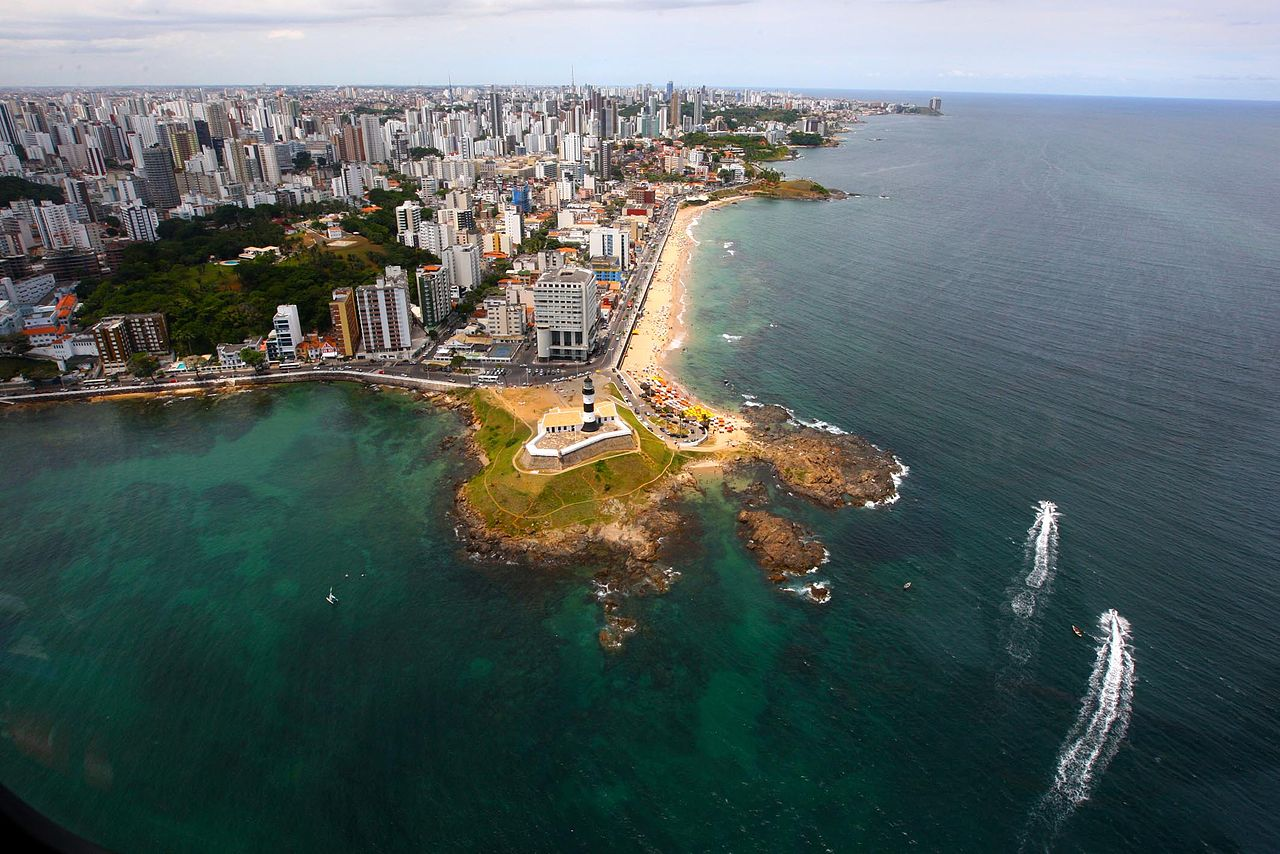
\includegraphics[width=0.45\textwidth]{images/farol_da_barra.jpg}
    \fol{hunter2007matplotlib}
    \label{fig:fig_exemplo_imagem3}
\end{figure}
\chapter{Conclusões}
\label{ch:conclusoes}

\textit{\textcolor{red}{Neste item o aluno deve apresentar as conclusões do estudo. As conclusões devem ser concisas e relacionadas com os objetivos propostos no trabalho.}}

\section{Sugestões para Trabalhos Futuros}
\label{section:sugestoes_trabalhos_futuros}

\textit{\textcolor{red}{Pode ainda, ao final, apresentar as perspectivas futuras do estudo.}}

% ----------------------------------------------------------
% ELEMENTOS PÓS-TEXTUAIS
% ----------------------------------------------------------
\postextual

% Referências bibliográficas
\bibliography{referencias/referencias.bib}

\end{document}